\chapter{Framework Implementation} \label{cha:implementation}
In this chapter the design of the \textbf{Hybrid Fortran} framework is presented from the implementation perspective. It will discuss the architecture that has been introduced for implementing the \textbf{Hybrid Fortran} framework, in order to achieve the goals and behaviour outlined in sec.~\ref{sec:frameworkGoals} and sec.~\ref{sec:archDirectives}. If you'd like to adjust the framework for your own purposes, this chapter is a good place to start.

\section{Overview and Build Workflow} \label{sub:buildSystem}

\begin{figure}[htpb]
	\centering
	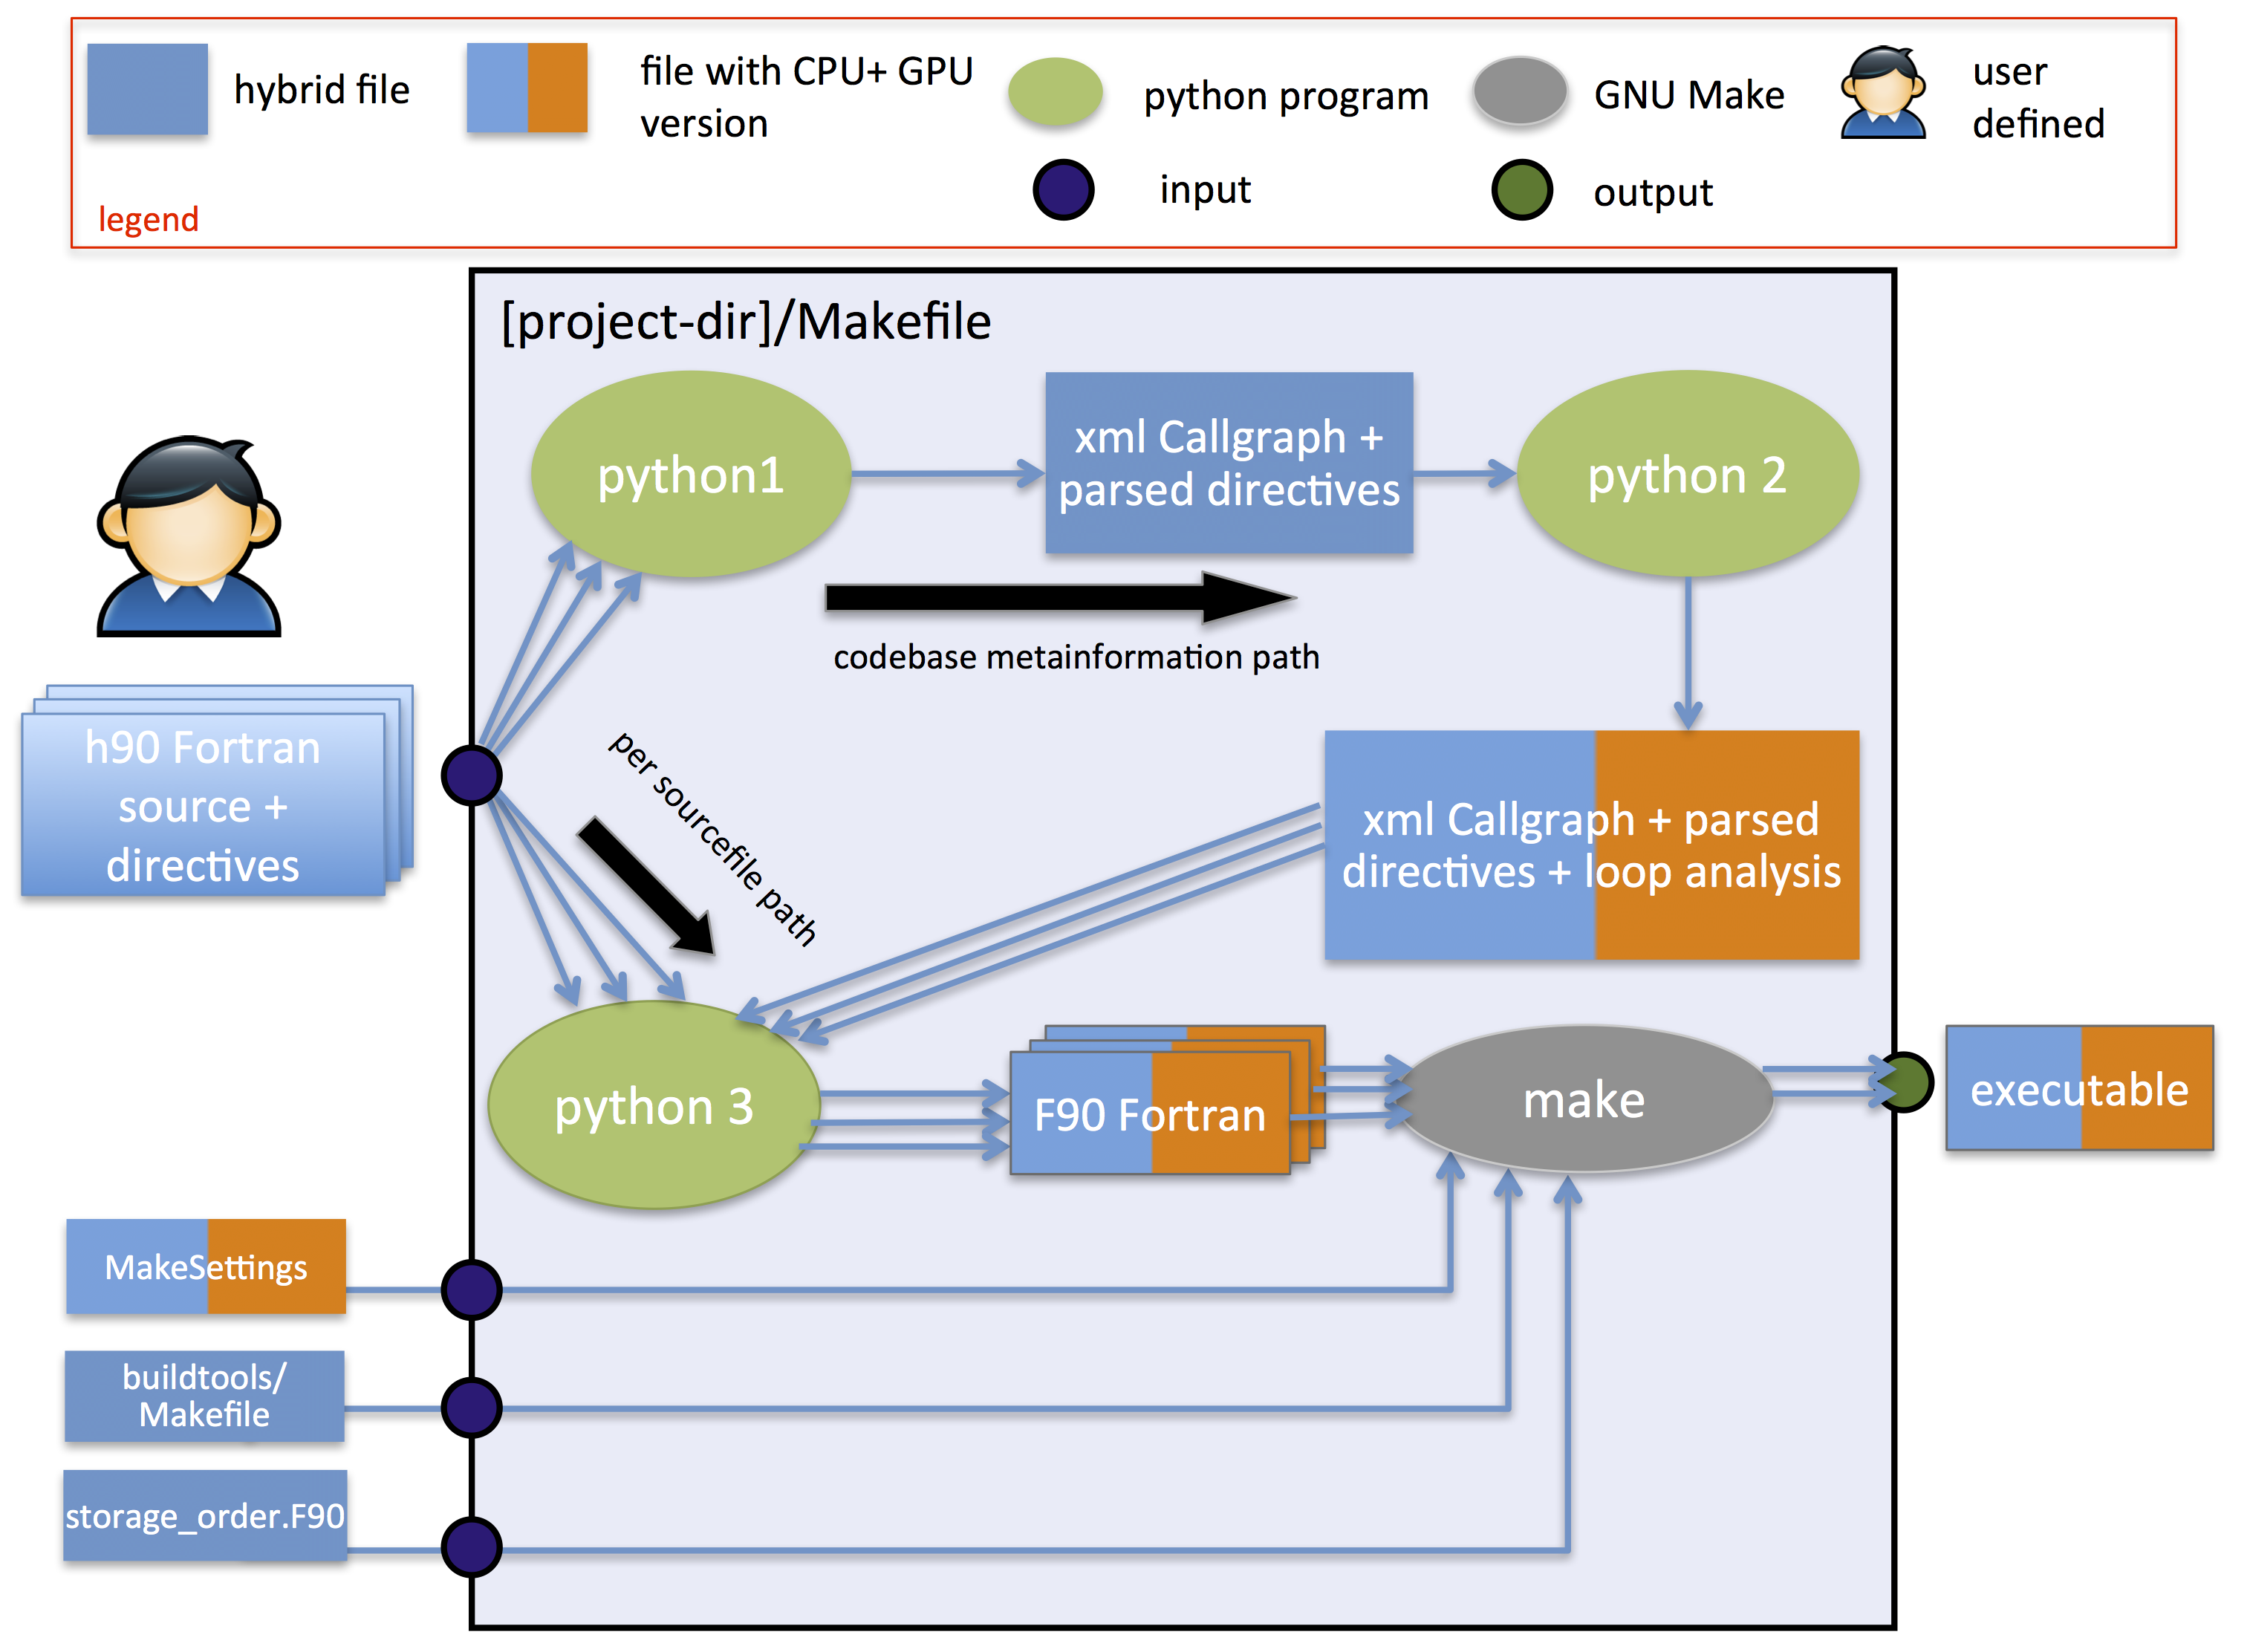
\includegraphics[width=14cm]{figures/hybridCUDAInformationFlow}
	\caption[Hybrid Fortran Components]{\textbf{Hybrid Fortran} Components and Information Flow.}
	\label{figure:hybridCUDAComponentsAndInfoFlow}
\end{figure}

The \textbf{Hybrid Fortran} build system involves the following components (depicted in fig.~\ref{figure:hybridCUDAComponentsAndInfoFlow}):

\begin{description}
 \item[project-dir/Makefile] offers a convenient interface to the build system. Please refer to appendix \ref{sub:buildInterface} for the usage of this build interface. It performs the following operations (assuming a clean rebuild):
 \begin{enumerate}
  \item Creates a build directory containing subdirectories for CPU and GPU builds.
  \item Copies all \verb|f90| and \verb|F90| source files (pure Fortran 90 sources without \textbf{Hybrid Fortran} directives) into the CPU and GPU build directories using a flat file hierarchy. 
  \item Creates the callgraph \verb|xml| file as well as the colored CPU and GPU callgraph versions in the callgraph subdirectory within the build directory.
  \item Creates the graphical callgraph representations in the callgraph directory using \textbf{Graphviz} libraries.
  \item Converts each \verb|h90| source file into \verb|F90| source files, using different implementations and callgraph colorings for the CPU and GPU case. The \verb|F90| files are created in their respective build subdirectories (CPU or GPU).
  \item Copies the \verb|project-dir/buildtools/Makefile| into the CPU and GPU source directories.
  \item Copies either \verb|project-dir/buildtools/MakesettingsCPU| and \linebreak
    \verb|project-dir/buildtools/MakesettingsGPU| into the respective build subdirectory.
  \item Executes \verb|make| within the build subdirectories.
  \item Installs the resulting executables into the test directory, using \verb|cpu| or \verb|gpu| as a postfix in the executable filename.
 \end{enumerate}
 \item[project-dir/buildtools/Makefile] defines the dependencies between the Fortran 90 and \textbf{Hybrid Fortran} sources. 
 \item[project-dir/buildtools/MakesettingsCPU] defines the compiler name, compiler flags and linker flags for the CPU case.
 \item[project-dir/buildtools/MakesettingsGPU] defines the compiler name, compiler flags and linker flags for the GPU case.
\end{description}

\begin{figure}[htpb]
	\centering
	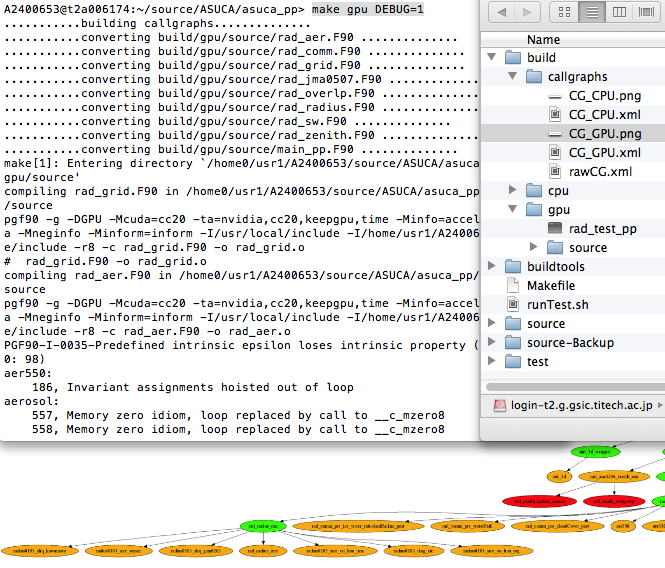
\includegraphics[width=10cm]{figures/uiScreenShot}
	\caption[Screenshot Build System]{Screenshot of the \textbf{Hybrid Fortran} build system in action.}
	\label{figure:buildSystemInAction}
\end{figure}

\section{Python Build Scripts} \label{sub:pythonScripts}

\noindent The following python command line interface programs are part of the \textbf{Hybrid Fortran} build system:

\begin{description}
 \item[annotatedCallGraphFromH90SourceDir.py] goes through all h90 files in a given source directory and builds an xml file containing meta information about that source tree. The extracted meta information includes the callgraph visible from h90 files as well as a parsed version of the \textbf{Hybrid Fortran} directives inserted by the user. Figure \ref{figure:hybridCUDAComponentsAndInfoFlow} depicts this program in node \verb|python 1|.
 \item[loopAnalysisWithAnnotatedCallGraph.py] takes the meta information xml file from the previous script as its input and analyses the positioning of the user defined parallel regions relative to all subprocedures. Depending on its input arguments it performs this analysis for either the CPU or GPU version of the program in order for the framework to support compile time defined positioning of loops (kernel regions in the CUDA implementation). Figure \ref{figure:hybridCUDAComponentsAndInfoFlow} depicts this program in node \verb|python 2|.
 \item[generateF90fromH90AndAnalyzedCallGraph.py] takes one h90 source file as well as the analyzed meta information xml file as its inputs. It goes through the source file line by line and rewrites it in order to create compatible versions for CPU and GPU. The following operations are most essential to this module: 
 \begin{itemize}
  \item Rewriting of parallel region definitions to conventional loops for the CPU or CUDA Fortran kernels for the GPU.
  \item Mutation of declarations and accesses of domain dependant arrays according to their position relative to the currently active parallel region.
  \item Insertion of statements to copy array data to and from the device in the GPU case.
 \end{itemize}
 Parallel domain dependant Figure \ref{figure:hybridCUDAComponentsAndInfoFlow} depicts this program in node \verb|python 3|.
 \item[graphVizGraphWithAnalyzedCallGraph.py] This program has been created in order to make debugging easier and to give the user an overview over the codebase and the involved parallel regions. It creates a graphical representation of the call graph from the analyzed meta information. The nodes in these call graphs are colored according to their relative position to the parallel regions. Figure \ref{figure:callgraph} shows a sample of such a programmatically created call graph representation.
\end{description}

\begin{figure}[htpb]
	\centering
	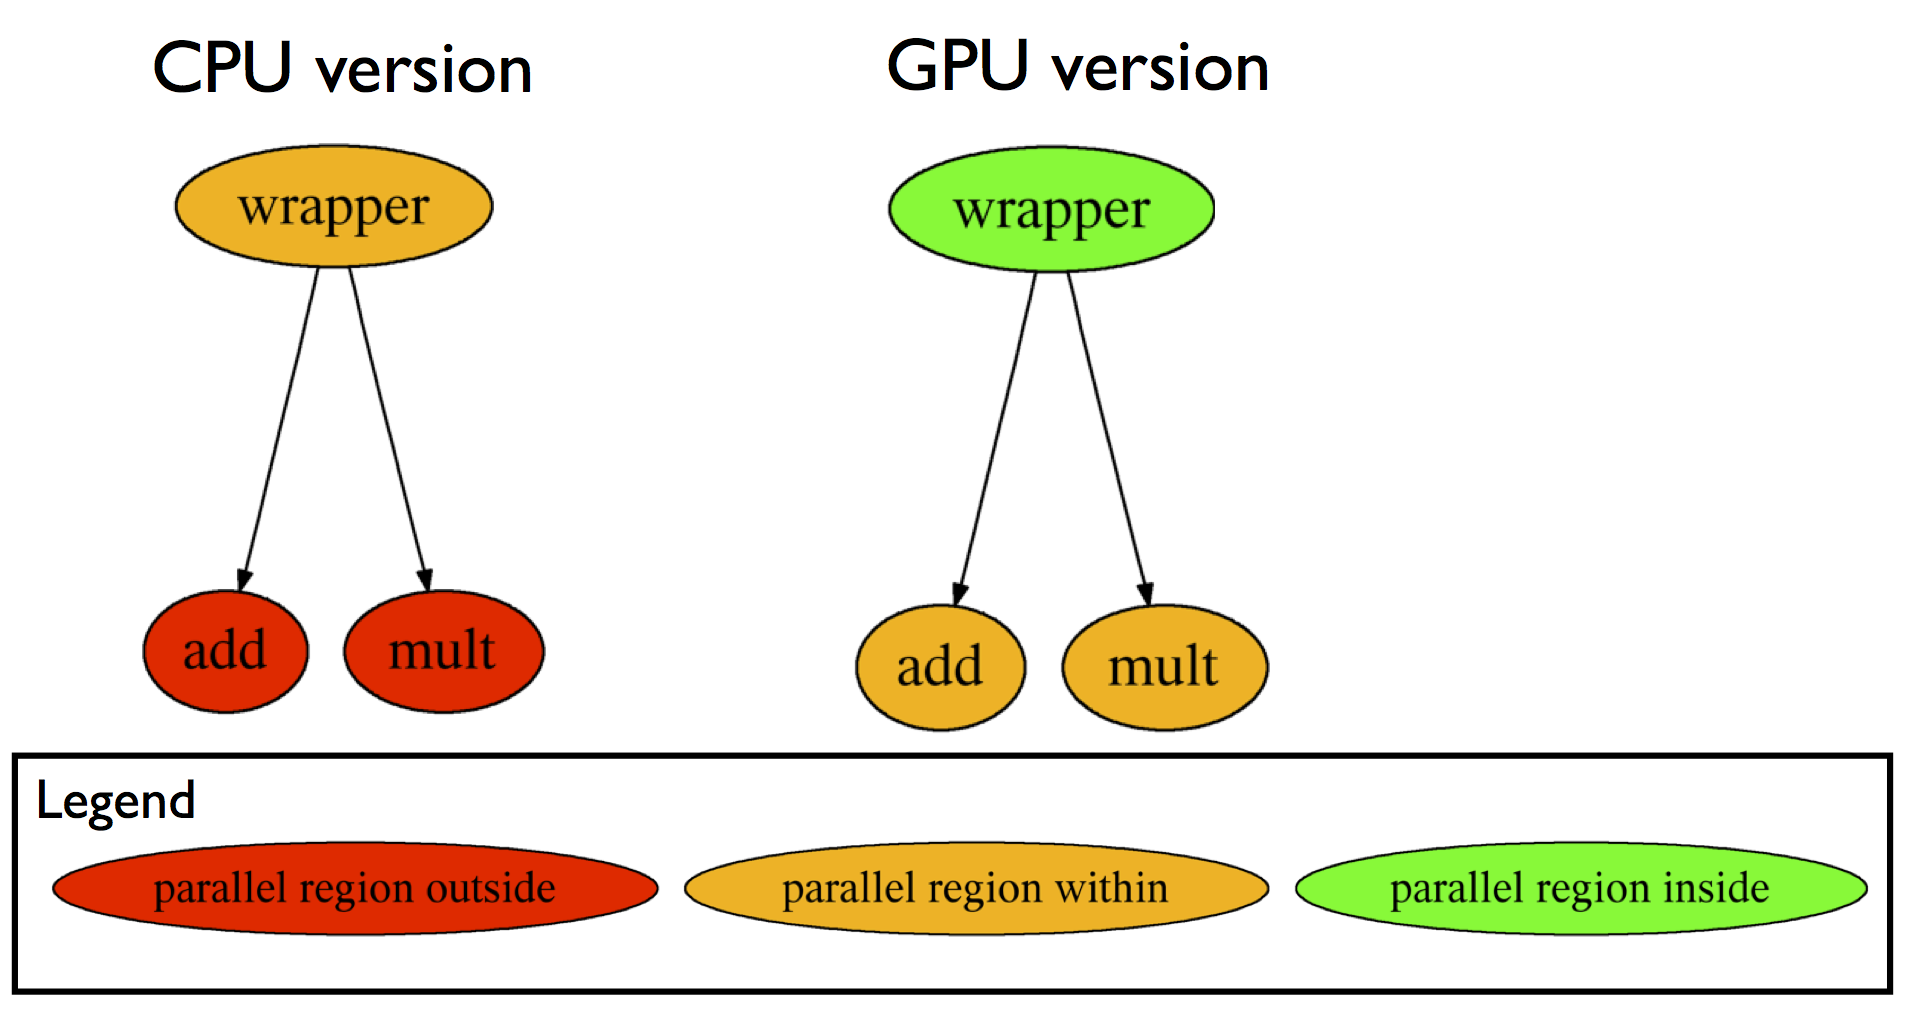
\includegraphics[width=10cm]{figures/callgraph}
	\caption[Callgraph Example]{Condensed version of a simple callgraph, programmatically created by graphVizGraphWithAnalyzedCallGraph.py.}
	\label{figure:callgraph}
\end{figure}

\section{User Defined Files} \label{sub:userDefinedFiles}

The following files, depicted figure \ref{figure:hybridCUDAComponentsAndInfoFlow}, are defined by the user:

\begin{description}
 \item[h90 Fortran sources] A source directory that contains \textbf{Hybrid Fortran} files (h90 extension). It may also contain files with f90 or F90 extensions. The source directory is by default located at \verb|path-to-project/source/*|.
 \item[Makefile] Used to define module dependencies. The Makefile is by default located at \verb|path-to-project/buildtools/Makefile|. Note: All source files are being copied into flat source folders before being compiled - the build system is therefore agnostic to the source directory structure implemented by the framework user.
 \item[storage\_order.F90] This fortran file contains fortran preprocessor statements in order to define the storage order for both CPU and GPU implementation. This file is located at
 \begin{verbatim*}path-to-project/source/
hybrid_fortran_commons/storage_order.F90.\end{verbatim*}

\end{description}

\section{Class Hierarchy} \label{sub:archHierarchy}

\begin{figure}[htpb]
	\centering
	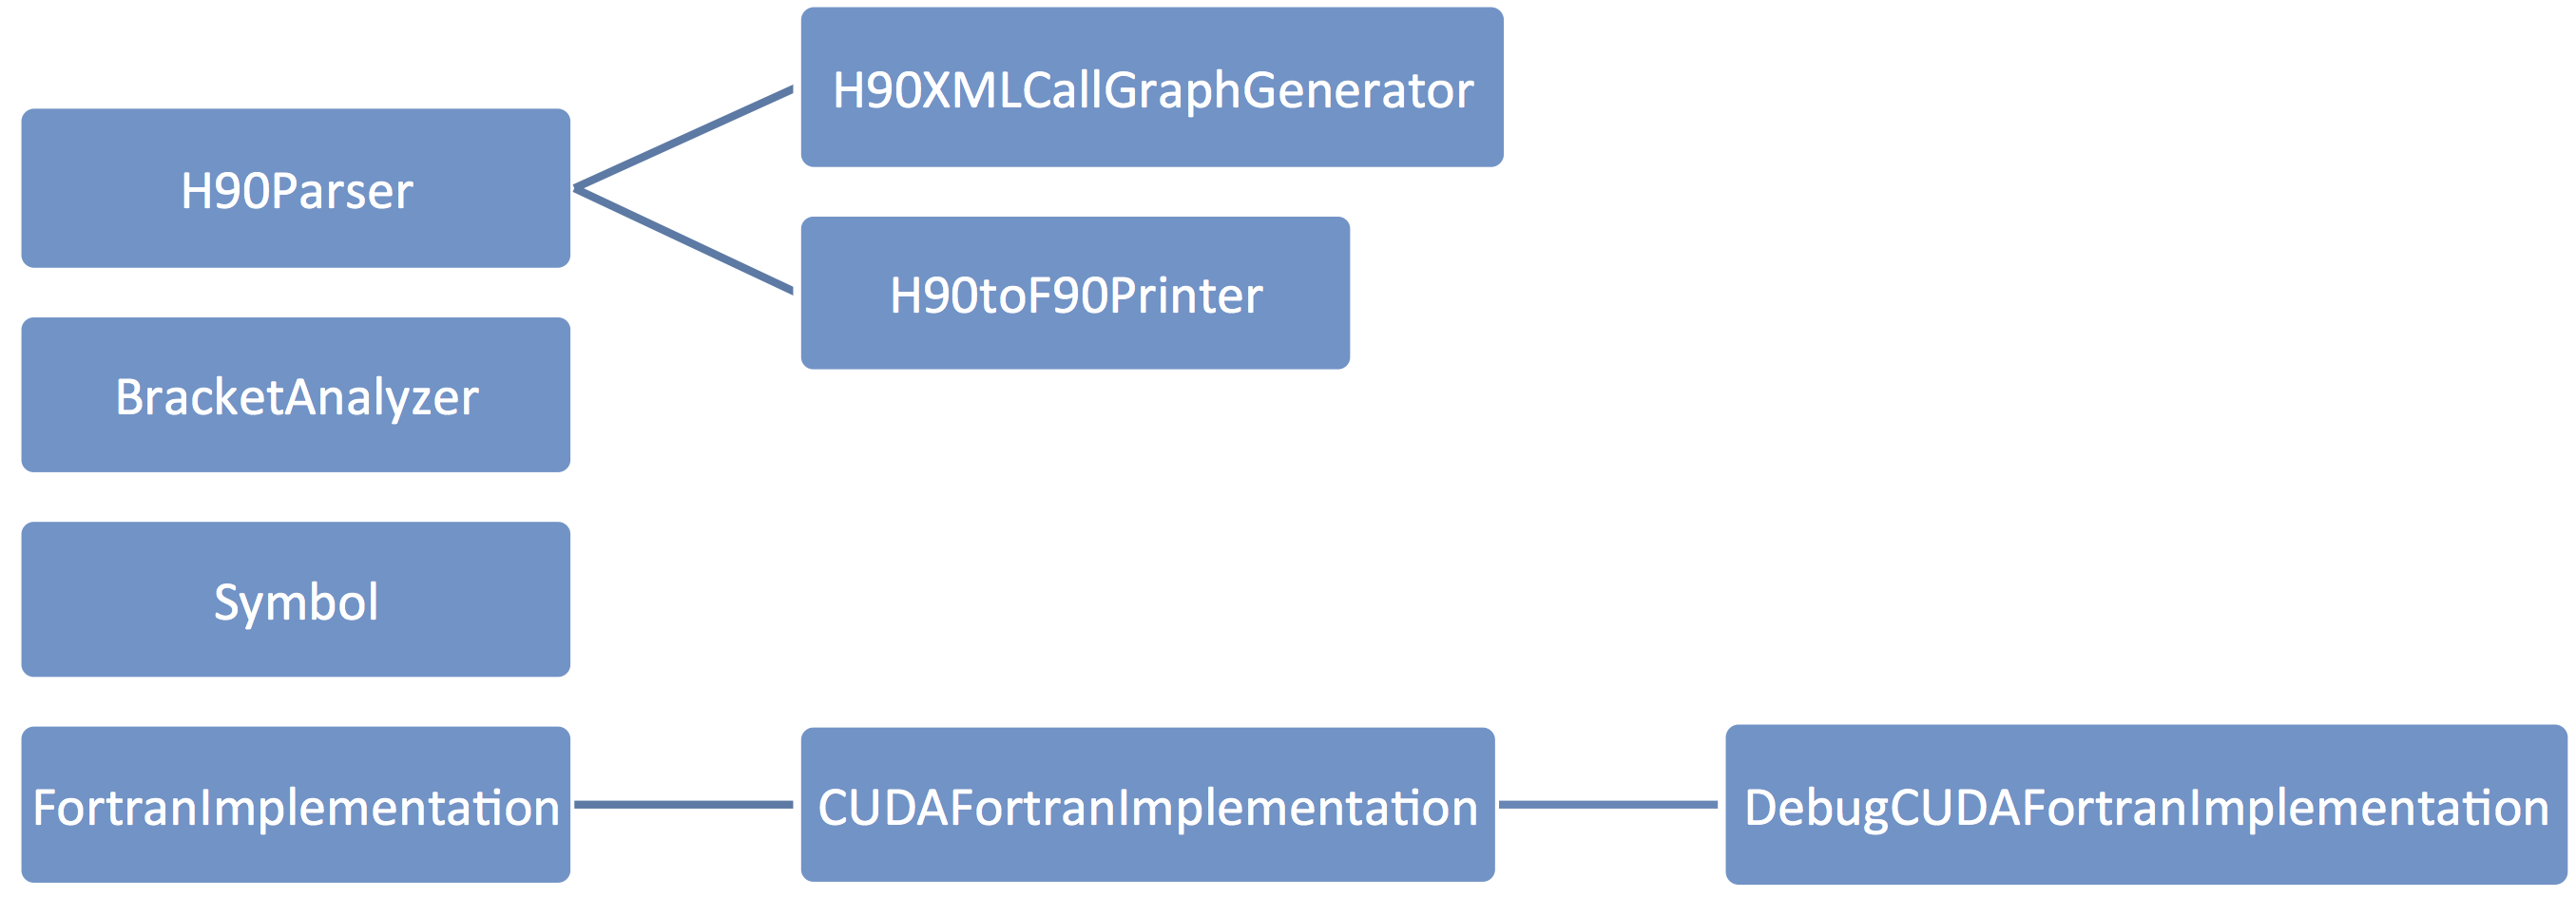
\includegraphics[width=14cm]{figures/classHierarchy}
	\caption[Hybrid Fortran Python Class Hierarchy]{\textbf{Hybrid Fortran} Python Class Hierarchy.}
	\label{figure:classHierarchy}
\end{figure}

Figure \ref{figure:classHierarchy} shows the classes created to implement the functionality described in section \ref{sub:pythonScripts}. For a full list of the implementation classes, please see also sec. \ref{sub:backendImplementation}.

\begin{description}
 \item[H90Parser] parses \textbf{Hybrid Fortran} (h90) files. The parser uses a mixture of state machine and regular expression design patterns. More specifically: Each line is matched against a set of regular expressions. The set of regular expressions being used is determined by a state machine and the outcomes of the regular expression matches in turn determine the state transitions. 
 See section \ref{sub:parser} for a more detailed look at the \textbf{Hybrid Fortran} parser implementation.
 \item[H90XMLCallGraphGenerator] (subclass of \verb|H90Parser|) adds routine and call nodes to a new or existing call graph xml document. This functionality is used by \linebreak 
 \verb|annotatedCallGraphFromH90SourceDir.py| as described in section \ref{sub:pythonScripts}. 
 \item[H90toF90Printer] (subclass of \verb|H90Parser|) prints a fortran 90 file in F90 format (including preprocessor statements) to POSIX standard output. The configuration of this class includes
  \begin{enumerate}
    \item a \textbf{Hybrid Fortran} file as its main input (inherited from the parent class).
    \item an xml callgraph including parsed \textbf{Hybrid Fortran} directives and the positions of parallel regions relative ot the routine nodes.
    \item a FortranImplementation object which determines the parallel implementation.
  \end{enumerate}
  \verb|generateF90fromH90AndAnalyzedCallGraph.py| uses this functionality as described in section \ref{sub:pythonScripts}.
 \item[BracketAnalyzer] is used to determine whether a Fortran line ends with an open bracket. 
 \item[Symbol] Stores array dimensions determined at the time of declaraton for later use and includes functionality to print adapted declaration and access statements.
 \item[FortranImplementation] provides the concrete syntax for a standard Fortran 90 implementation of the \textbf{Hybrid Fortran} program.
 \item[CUDAFortranImplementation] (subclass of \verb|FortranImplementation|) provides the syntax for a CUDA Fortran implementation, thus handling 
 \begin{itemize}
  \item the conversion of parallel region directives into CUDA kernels,
  \item the conversion of subroutines called by kernels into device subroutines,
  \item the copying of data from and to the device,
  \item the synchronization of threads after CUDA kernels have finished executing (asynchronous execution of kernels is currently not supported) and
  \item error handling.
 \end{itemize}
 \item[DebugCUDAFortranImplementation] (subclass of \verb|CUDAFortranImplementation|) extends the CUDA Fortran implementation to include print statements to POSIX standard error output for all kernel parameters at a user defined data point after the execution of the kernel. This functionality enables debugging of device code since barebone CUDA Fortran currently does not offer printing or debugging for code executed on the GPU. (There is an emulation mode available which runs CUDA Fortran programs on the CPU, however it has been found to diverge too much from the device version).
\end{description}

\section{Switching Implementations} \label{sub:switchImplementation}

Figure \ref{figure:implementationMap} shows the the most important class member functions of \linebreak
\verb|FortranImplementation| classes and their role with respect to the example shown earlier in section \ref{sub:directiveExample}. Each of these methods takes context information objects (for example a set of symbols that are referenced on this line, or a parallel region template containing the information users have passed with the directives) and returns strings that will be inserted at the indicated places into Fortran 90 files by the \verb|H90toF90Printer| class. Introducing a new underlying technology such as OpenCL (for GPU implementations) or OpenMP (for CPU implementations) is as simple as writing a new \verb|FortranImplementation| subclass containing these functions. 

\begin{figure}[htpb]
	\centering
	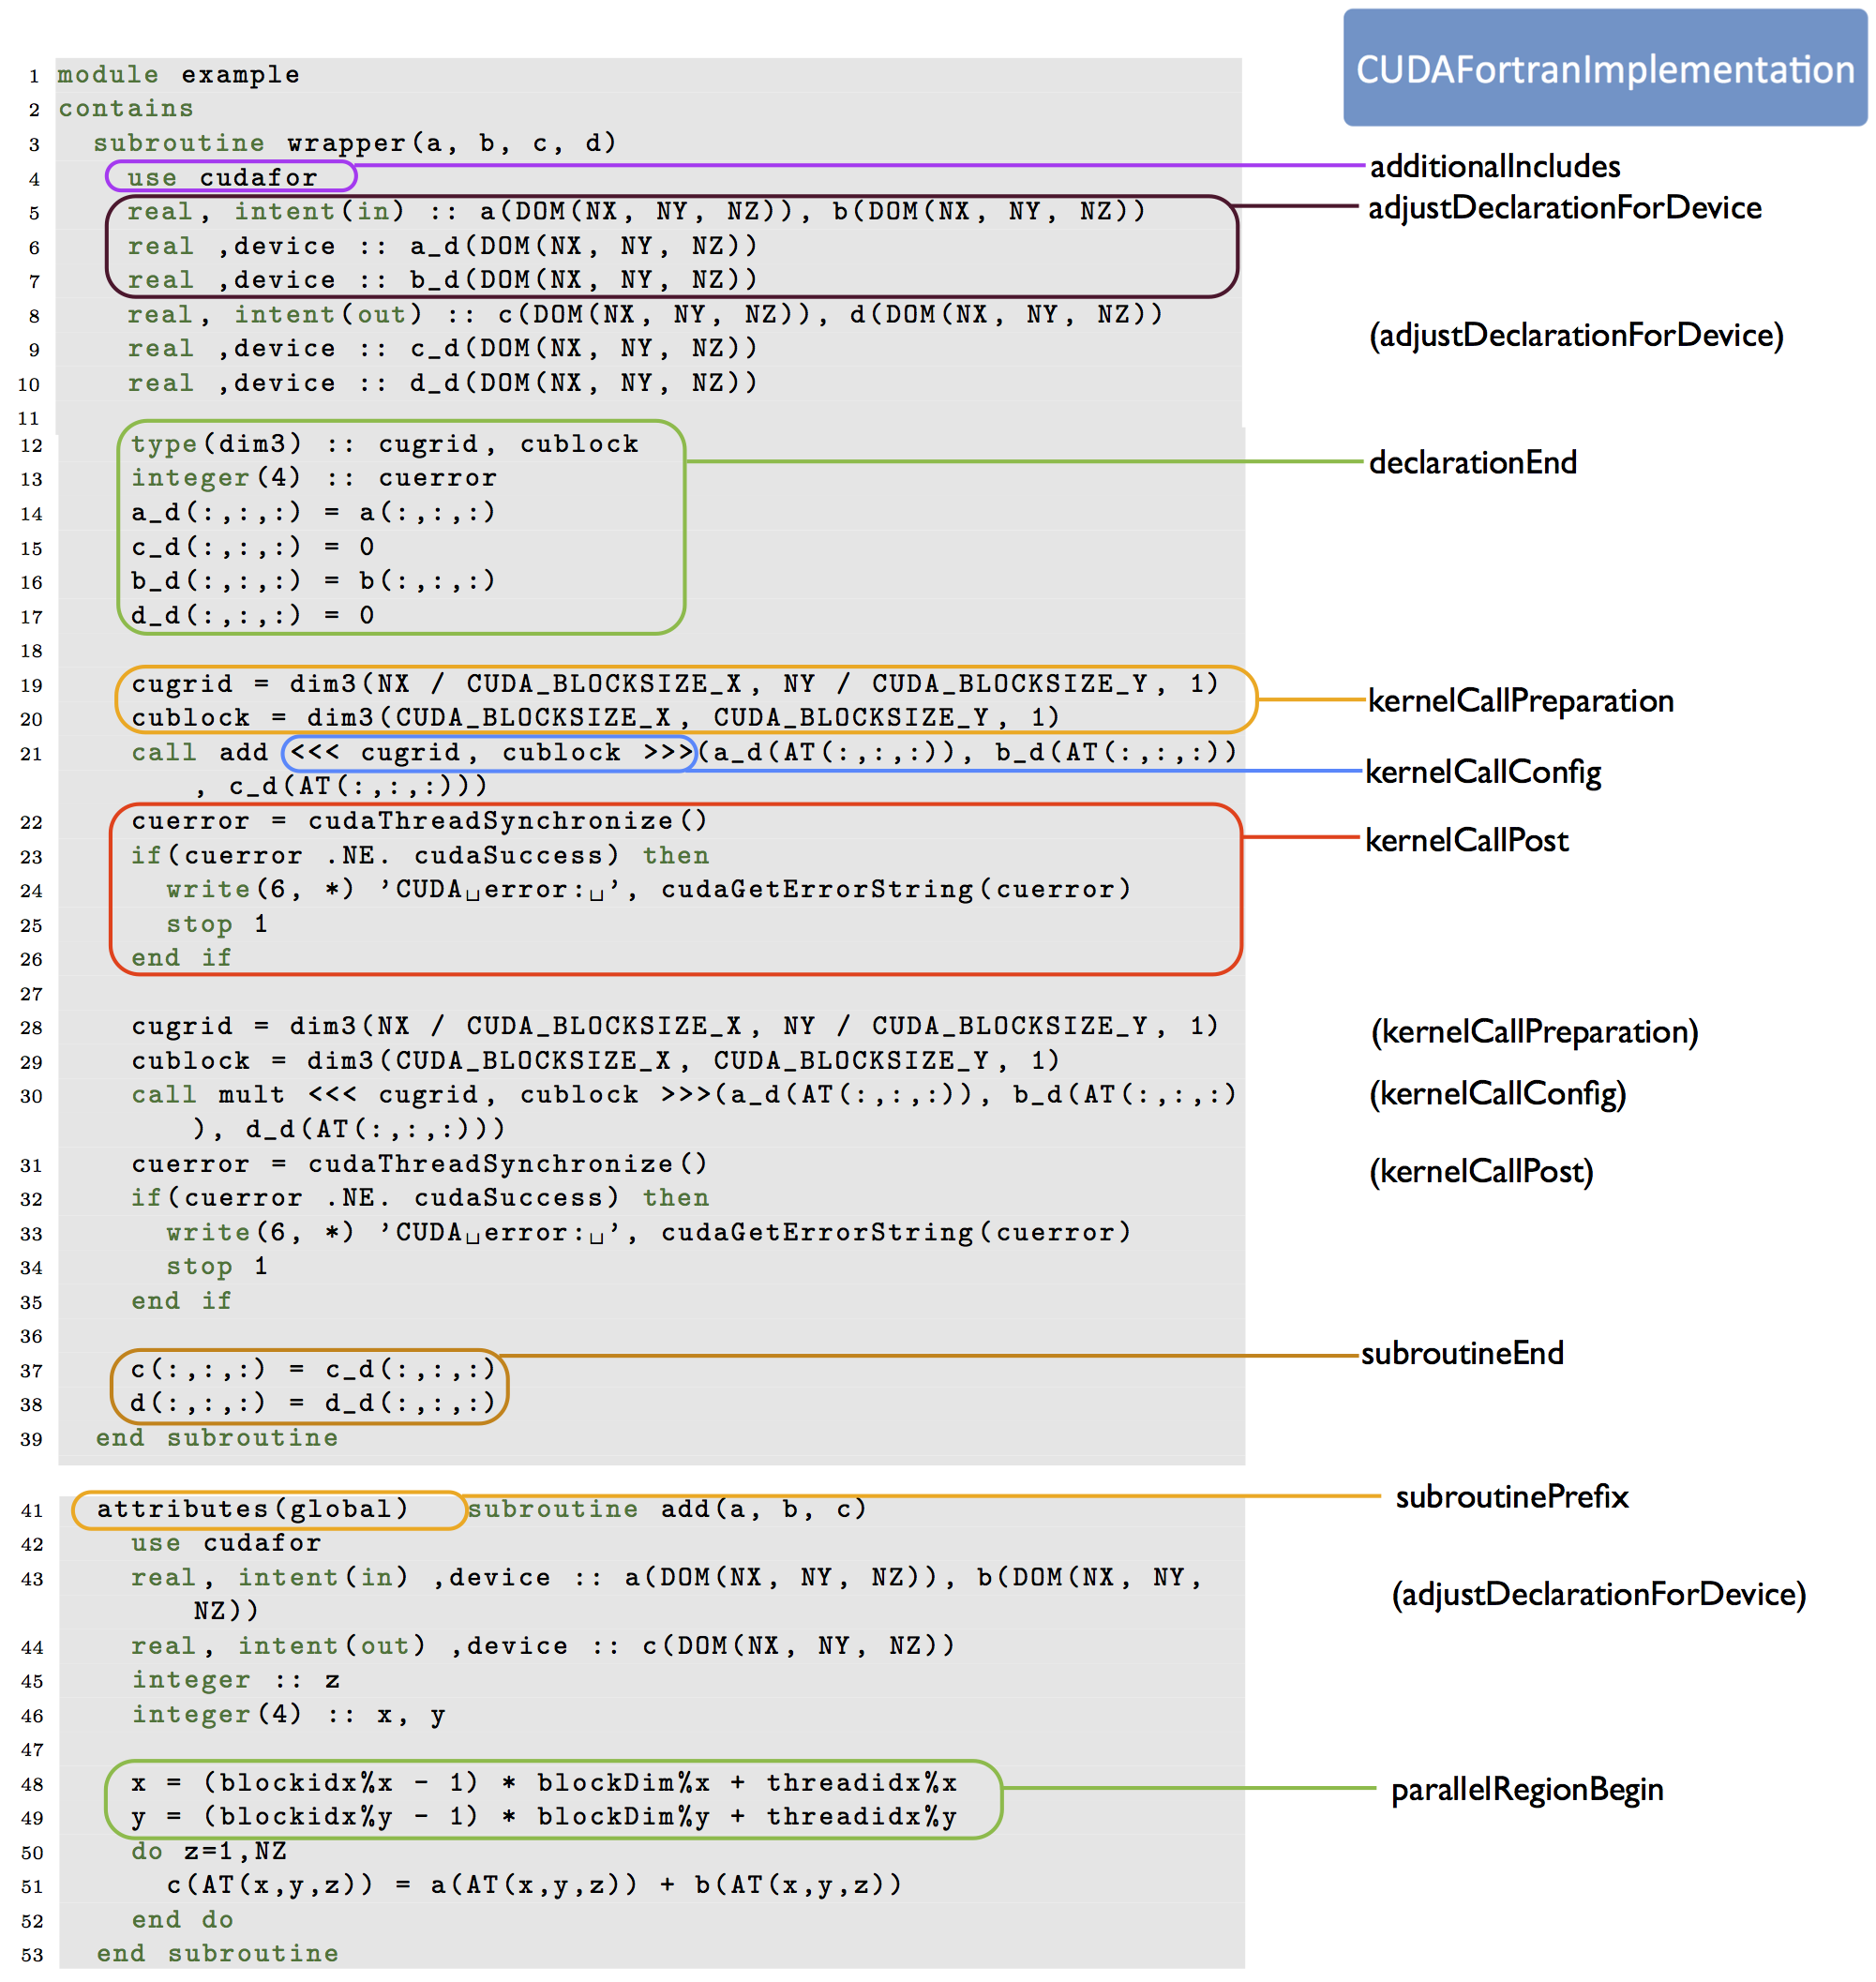
\includegraphics[width=12cm]{figures/implementationMap}
	\caption[Switching Fortran Implementations]{Class member functions of ``FortranImplementation'' classes (Example shown with CUDAFortranImplementation).}
	\label{figure:implementationMap}
\end{figure}
\clearpage

\section{Hybrid Fortran Parser} \label{sub:parser}

In order to interpret the directives introduced in cha~\ref{cha:framework} in the right context, it was necessary to create the parser program outlined in this section. This parser is used by the \verb|annotatedCallGraphFromH90SourceDir| and \linebreak \verb|generateF90fromH90AndAnalyzedCallGraph.py| python scripts (as described in sec.~\ref{sub:pythonScripts}) through subclasses. 

This section gives a more detailed view of that parser. Figure \ref{figure:parserStateMachine} shows the state machine pattern that has been used for the parser implementation.

\begin{figure}[htpb]
	\centering
	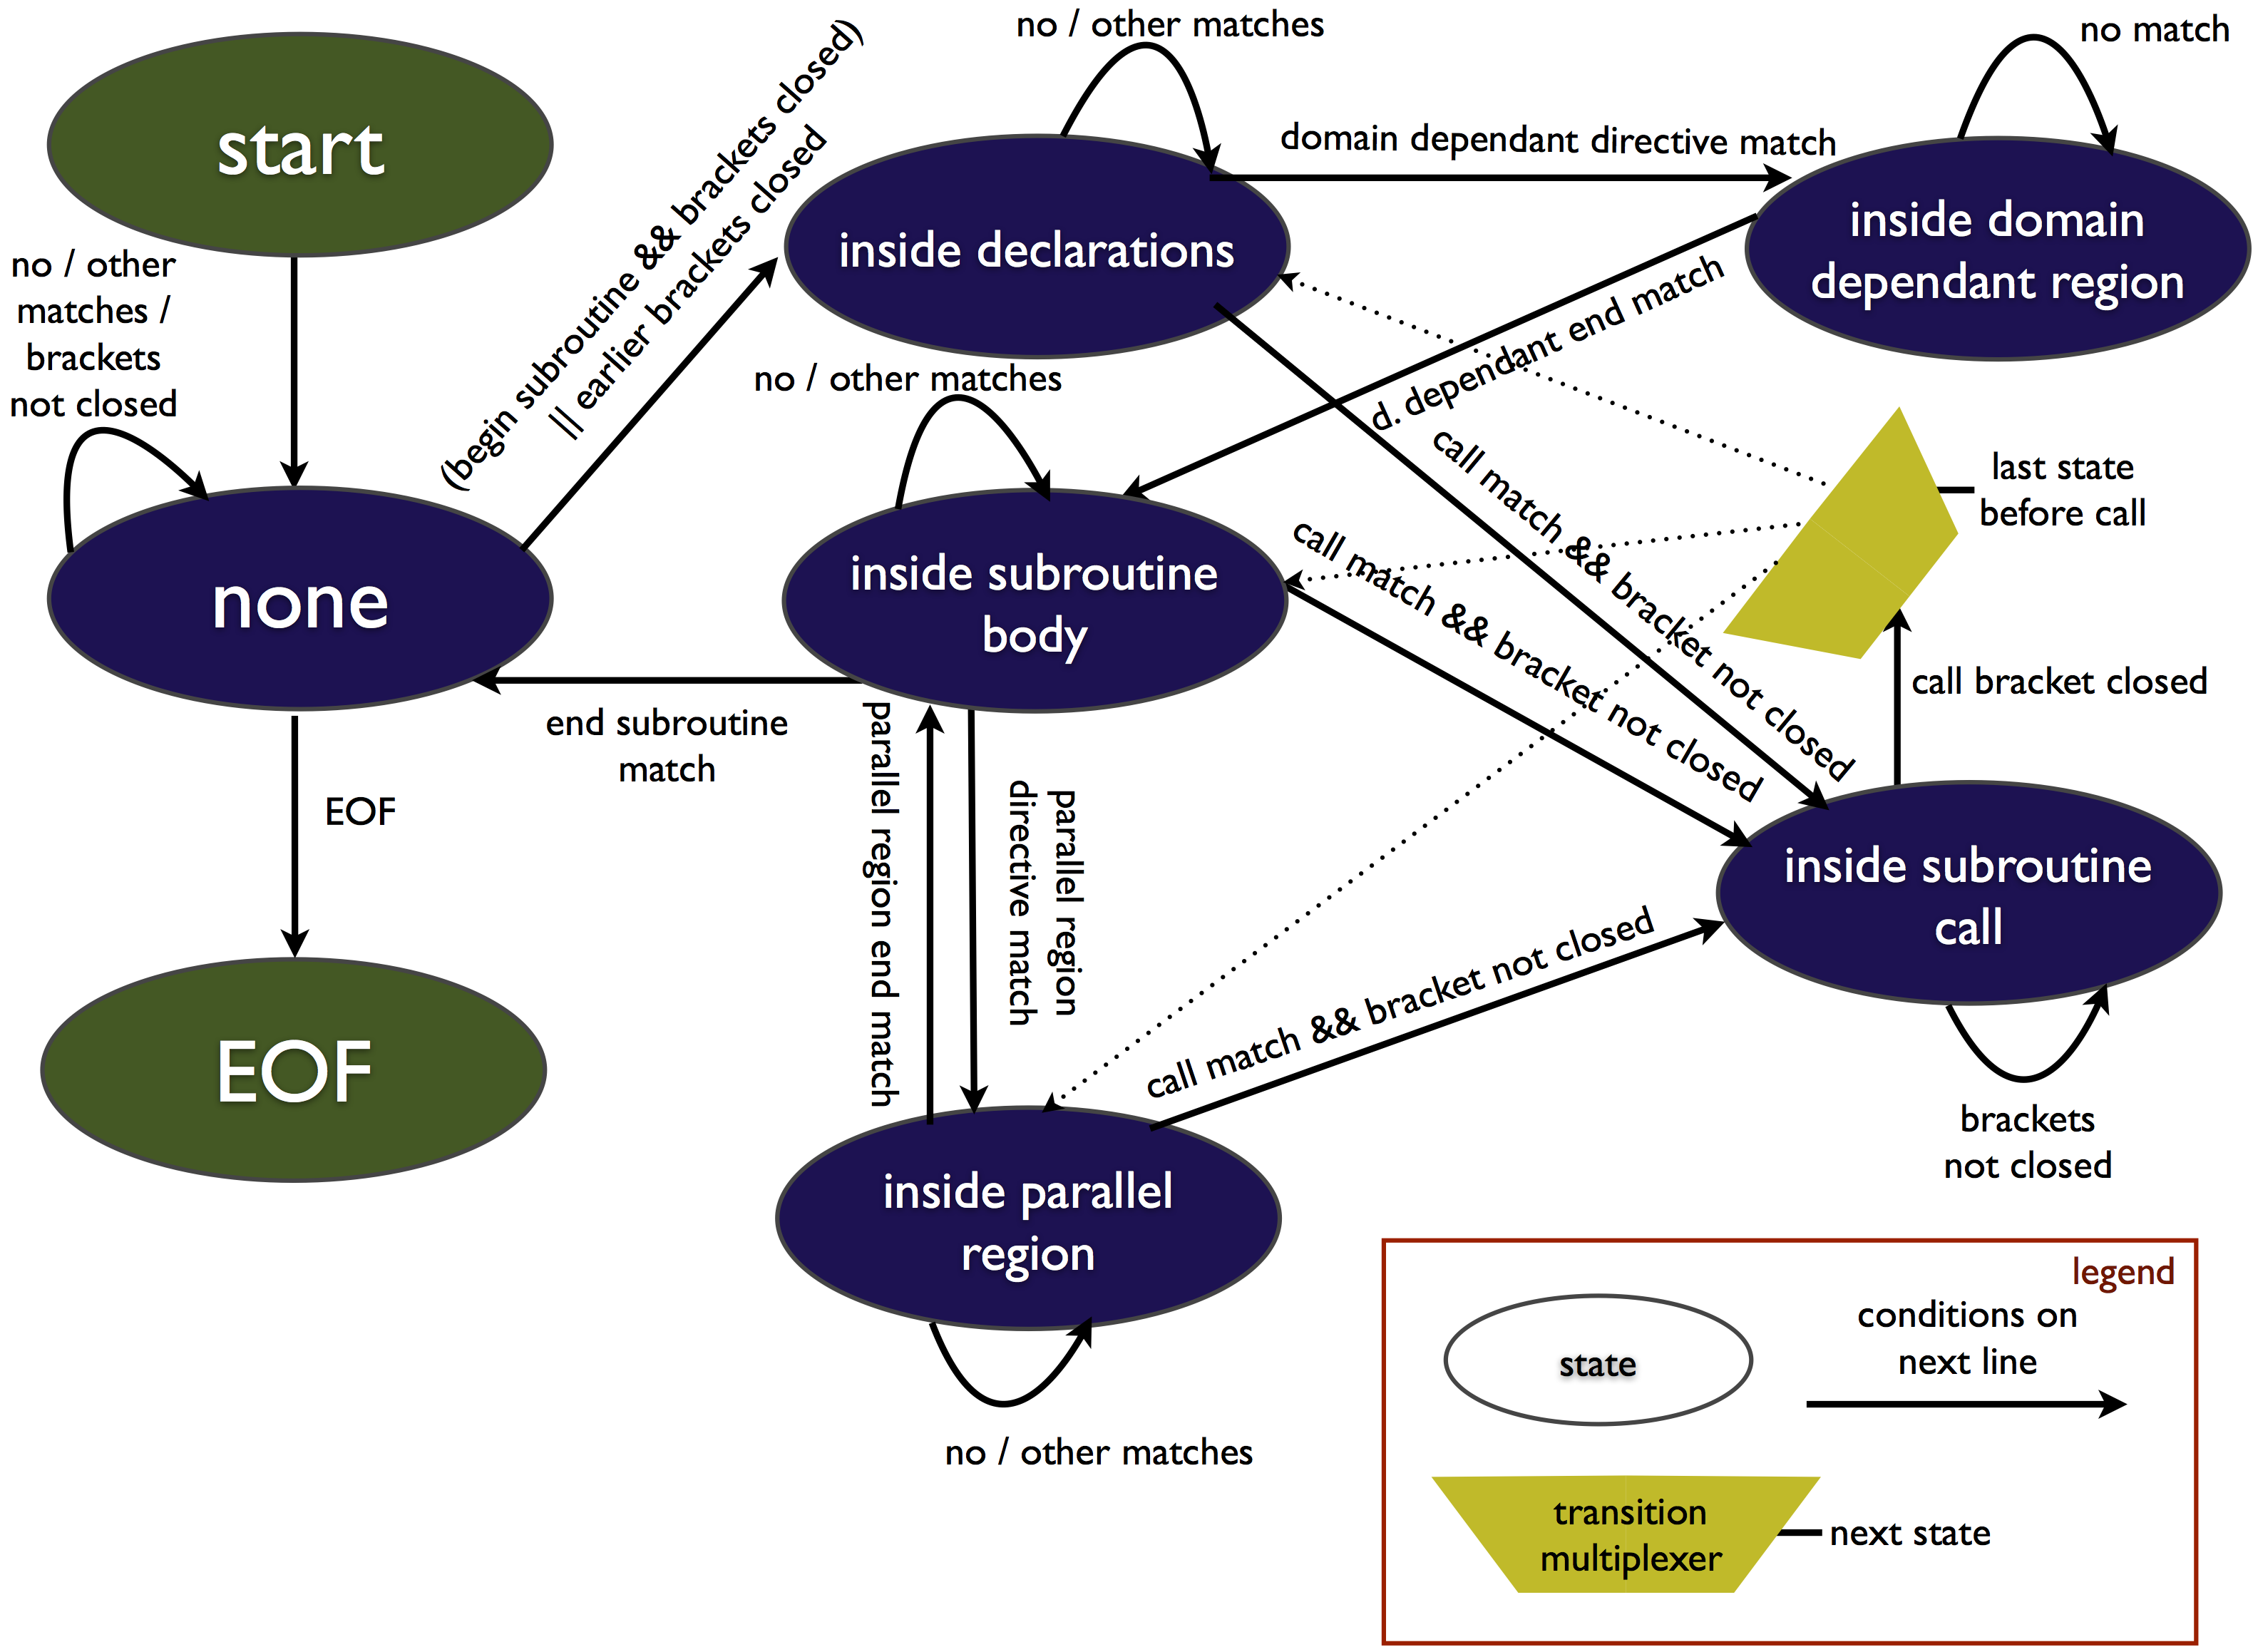
\includegraphics[width=14cm]{figures/parserStateMachine}
	\caption[Parser State Machine]{H90 Parser State Machine.}
	\label{figure:parserStateMachine}
\end{figure}

The state machine design pattern being used here resembles that of a Mealy machine. However, two changes have been applied to the Mealy machine properties:
\begin{enumerate}
  \item The output is being detached from the machine. In other words the \verb|H90Parser| class does not produce any output itself. Its subclasses (as described in sec.~\ref{sub:archHierarchy}) are responsible for that task. This allows large parts of the parser code to be reused for both python programs dealing with h90 source files as described in sec.~\ref{sub:pythonScripts}
  \item A multiplexer is introduced as an additional element in order to reduce the number of states (which matches the way code is being reused in the actual implementation).
\end{enumerate}
 
% Listing \ref{listing:parserImplementation} gives a simplified overview of how the parser is implemented in code. A few notes: 
% \begin{enumerate}
%  \item The matchings are implemented using regular expressions as mentioned in section \ref{sub:archHierarchy}. 
%  \item Since python does not have a \verb|switch case| statement, a dictionary has been used instead (functions by state).
%  \item The bracket handling is actually wrapped in its own class (\verb|BracketAnalyzer|) as mentioned in section \ref{sub:archHierarchy}. 
% \end{enumerate}
% 
% 
% \begin{lstlisting}[name=parserImplementation, label=listing:parserImplementation]
%   bracketState = 0
%   state = none
%   stateBeforeCall = none
%   
%   function processNoneState(nextLine):
%     if nextLine matches subroutine beginning 
%     OR bracketState != 0:
%       /* analyseBracketState will return        */
%       /* the bracket level after nextLine       */
%       /* e.g. if all brackets have been closed, */
%       /* it will return 0                       */
%       bracketState = analyseBracketState(
% 			nextLine, bracketState
% 		     )
%       if bracketState == 0:
% 	processSubroutineMatch(match)
% 	state = inside_declarations
%       return
%       
%   function processInsideDeclarationsState(nextLine):
%     if nextLine matches beginning 
%     of domain dependant region:
%       processDomainDependantRegionMatch(match)
%       state = inside_domainDependantRegion
%     else if nextLine matches subroutine call:
%       processSubroutineCallMatch(match)
%       bracketState = analyseBracketState(
% 			nextLine, bracketState
% 		     )
%       if bracketState != 0:
% 	stateBeforeCall = state
% 	state = inside_subroutine_call
% 	
%   function process[...]State(nextLine):
%     ... 
%     
%   while EOF has not been reached:
%     nextLine = next line from current h90 file
%     choose state:
%       case none:
% 	processNoneState(nextLine)
%       case inside_declarations:
% 	processInsideDeclarationsState(nextLine)
%       case inside_domainDependantRegion:
% 	processInsideDomainDependantRegionState(nextLine)
%       case inside_subroutine_body:
% 	processInsideSubroutineBodyState(nextLine)
%       case inside_parallelRegion
% 	processInsideParallelRegionState(nextLine)
%       case inside_subroutine_call:
% 	processInsideSubroutineCallState(nextLine)
% \end{lstlisting}
